\chapter{Μεθοδολογία}
\label{ch:methodology}

\section{Στοιχειώδεις Γεωμετρικές Πράξεις}
\subsection{Ευκλείδεια Απόσταση δύο Τριγώνων}
\label{subsec:tria_distance}
% Έστω τα τρίγωνα $P$ και $Q$ στον $\mathbb{R}^3$.
% Η Ευκλείδεια απόσταση $d(P,Q)$ μεταξύ των τριγώνων $P$ και $Q$
% ορίζεται ως:
% \[ d(P,Q) = \min_{p \in P, q \in Q} |p - q| \]
% όπου με $|p-q|$ συμβολίζεται η Ευκλείδεια απόσταση των σημείων 
% $p$ και $q$.

% Έστω p,q

\subsubsection{Ευκλείδεια Απόσταση δύο Ευθυγράμμων Τμημάτων}
\subsubsection{Ευκλείδεια Απόσταση Σημείου και Τριγώνου}

\subsection{Ευκλείδεια Απόσταση δύο \tl{AABB}}
Έστω τα ευθυγραμμισμένα με τους άξονες πλαίσια
$P$ και $Q$ στον $\mathbb{R}^3$.
Η Ευκλείδεια απόσταση $d(P,Q)$ μεταξύ των πλαισίων $P$ και $Q$
ορίζεται ως:
\[ d(P,Q) = \min_{p \in P, q \in Q} \lVert p - q \rVert \]
όπου με $\lVert p - q \rVert$ συμβολίζεται η Ευκλείδεια 
απόσταση των σημείων $p$ και $q$.

Ένα \tl{AABB} αναπαριστάται στη μνήμη από τα άκρα της κύριας 
διαγωνίου του.
Δηλαδή το σημείο $S$ με τις μικρότερες $x$, $y$, $z$ συντεταγμένες
και το σημείο $T$ με τις μεγαλύτερες $x$, $y$, $z$ συντεταγμένες.

\begin{figure}[h]
    \centering
    
    \newcommand{\Depth}{2}
    \newcommand{\Height}{2}
    \newcommand{\Width}{3}
    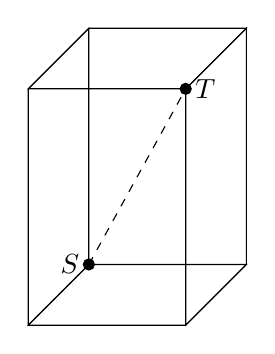
\begin{tikzpicture}
        \coordinate (O) at (0,0,0);
        \coordinate (A) at (0,\Width,0);
        \coordinate (B) at (0,\Width,\Height);
        \coordinate (C) at (0,0,\Height);
        \coordinate (D) at (\Depth,0,0);
        \coordinate (E) at (\Depth,\Width,0);
        \coordinate (F) at (\Depth,\Width,\Height);
        \coordinate (G) at (\Depth,0,\Height);

        \draw[] (O) -- (C) -- (G) -- (D) -- cycle;% Bottom Face
        \draw[] (O) -- (A) -- (E) -- (D) -- cycle;% Back Face
        \draw[] (O) -- (A) -- (B) -- (C) -- cycle;% Left Face
        \draw[] (D) -- (E) -- (F) -- (G) -- cycle;% Right Face
        \draw[] (C) -- (B) -- (F) -- (G) -- cycle;% Front Face
        \draw[] (A) -- (B) -- (F) -- (E) -- cycle;% Top Face

        \draw[fill=black] (O) circle (2pt) node[left]{$S$};
        \draw[fill=black] (F) circle (2pt) node[right]{$T$};
        \draw[dashed] (O) -- (F);
    \end{tikzpicture}
    \caption[Αναπαράσταση ενός \tl{AABB}]{Αναπαράσταση ενός \tl{AABB}}
\end{figure}


Για τον υπολογισμό της απόστασης μεταξύ δύο τέτοιων πλαισίων, 
εκμεταλλευόμαστε το γεγονός ότι οι πλευρές τους είναι ευθυγραμμισμένες
με του άξονες.
Έτσι μπορούμε να υπολογίσουμε την απόσταση χωρίζοντας τη στις συνιστώσες της.
Τελικά, προκύπτει ο αλγόριθμος \ref{alg:aabb_dist}, 
όμοιος με αυτόν που περιγράφεται στο \cite{krishnamurthy2011gpu}.
Στον παραπάνω αλγόριθμο  ο τελεστής "$-$" στις γραμμές 
$1$,$2$ είναι διανυσματική αφαίρεση των συντεταγμένων των σημείων.
Ο τελεστής \tl{\texttt{max(0, $v$)}} είναι επίσης διανυσματικός και
αντικαθιστά όλες τις αρνητικές τιμές ενός διανύσματος $v$
με $0$.

\selectlanguage{english}
\IncMargin{1.5em}
\begin{algorithm}[h]
    \DontPrintSemicolon
    \KwIn{Two AABBs $P$, $Q$}
    \KwOut{Euclidean Distance of $P$ and $Q$}
    \SetKwFunction{funcname}{AABB\_distance}
    \SetKwFunction{max}{max}
    \Indm\nonl\funcname($P$, $Q$)\\
    \Indp
        $w \gets \max(0, P.S - Q.T)$\;
        $v \gets \max(0, Q.S - P.T)$\;
        \Return{$\sqrt{v \cdot v + w \cdot w}$}

    \caption[Υπολογισμός Απόστασης δύο \tl{AABB}]{
        \tg{Υπολογισμός της Ευκλείδειας Απόστασης δύο AABB}
    }
    \label{alg:aabb_dist}
\end{algorithm}
\DecMargin{1.5em}
\selectlanguage{greek}

\section{Αλγόριθμοι Εξαντλητικής Αναζήτησης}
\label{sec:exhaustive_search}
Έστω δύο αντικείμενα του τρισδιάστατου χώρου που αναπαρίστανται από 
τριγωνικά πλέγματα.
Από τον ορισμό της Ευκλείδειας απόστασης δύο τριγωνικών πλεγμάτων που
δόθηκε στην ενότητα \ref{sec:problem_description} και τη χρήση μιας 
ρουτίνας \tl{\texttt{triangle\_distance(p, q)}}, προκύπτει ο 
τετριμμένος αλγόριθμος \ref{alg:exhaustive_search}. 
Η πολυπλοκότητα του αλγορίθμου είναι $\bigO(N*M)$, όπου 
$N$ και $M$ είναι το πλήθος των τριγώνων των δύο αντικειμένων.

\selectlanguage{english}
\IncMargin{1.5em}
\begin{algorithm}[h]
    \DontPrintSemicolon
    \KwIn{Two Triangle Meshes $P$, $Q$}
    \KwOut{Euclidean Distance of $P$ and $Q$}
    \SetKwFunction{dist}{triangle\_distance}
    \SetKwFunction{trias}{triangles}
    \SetKwFunction{min}{min}
    \SetKwFunction{exhaustivesearch}{triangle\_mesh\_distance}
    \Indm\nonl\exhaustivesearch ($P$, $Q$)\\
    \Indp
        $T_P \gets$ \trias($P$) \;
        $T_Q \gets$ \trias($Q$) \; 
        $distance \gets \inf$ \;
        \ForEach{$p \in T_P$}{
            \ForEach{$q \in T_Q$}{
                $distance \gets \min(distance, \dist(p,q))$\;
            }
        }
        \Return{$distance$}

    \caption[Απόσταση Τριγωνικών Πλεγμάτων με Πλήρη Αναζήτηση]{
        \tg{Απόσταση Τριγωνικών Πλεγμάτων με Πλήρη Αναζήτηση}
    }
    \label{alg:exhaustive_search}
\end{algorithm}
\DecMargin{1.5em}
\selectlanguage{greek}

Σύμφωνα με τη μελέτη που έγινε στην ενότητα \ref{sec:bounding_volumes}
μπορούμε να επιταχύνουμε τον χρόνο εκτέλεσης του αλγορίθμου αν 
χρησιμοποιήσουμε οριοθετικούς όγκους.
Συγκεκριμένα, θα χρησιμοποιήσουμε Οριοθετικά Πλαίσια Ευθυγραμμισμένα 
με τους Άξονες (\tl{AABB}). 
Όπως φαίνεται από τον πίνακα της ενότητας \ref{sec:geom_tests_cost},
ο υπολογισμός της ελάχιστης απόστασης \textit{\tl{AABB - AABB}} είναι πολύ πιο 
"οικονομικός" υπολογιστικά σε σχέση με τον υπολογισμό της απόστασης 
\textit{τρίγωνο - τρίγωνο}.
Μπορούμε να εκμεταλλευτούμε αυτό το γεγονός και σε συνδυασμό με το παρακάτω λήμμα 
να σχεδιάσουμε έναν ταχύτερο αλγόριθμο.

\begin{lemma}
    Έστω δύο σύνολα $S_A$ και $S_B$ που αποτελούνται από χωρικά αντικείμενα. 
    Έστω οι οριοθετικοί όγκοι $BV_A$ και $BV_B$ που εξ' ολοκλήρου περικλείουν 
    τα αντικείμενα των σύνολων  $S_A$ και $S_B$, αντίστοιχα. Τότε:
    
    \[ distance(BV_A, BV_B) \leq distance(a, b) , 
    \forall a \in S_A, \forall b \in S_B \]

    Δηλαδή, η Ευκλείδεια απόσταση οποιουδήποτε ζεύγους αντικειμένων από τα δύο σύνολα 
    θα είναι μεγαλύτερη η ίση με την Ευκλείδεια των οριοθετικών όγκων των συνόλων.
    \label{lemma:box_distance}
\end{lemma}


\begin{proof}
    Συμβολίζουμε με $BV_A$ το σύνολο των σημείων του 
    οριοθετικού όγκου, $BV_A$. 
    Όμοια και για το σύνολο $BV_B$.

    Επίσης, έχουμε
    $S_A = \bigcup\limits_{a \in S_A} a $ και $S_B = \bigcup\limits_{b \in S_B} b$,
    όπου με $a$, $b$ συμβολίζουμε το σύνολο των σημείων των 
    χωρικών αντικειμένων $a$ και $b$.

    Αφού οι οριοθετικοί όγκοι περικλείουν τα σύνολα των 
    αντικειμένων $S_A$ και $S_B$ ισχύει επίσης ότι 
    $S_A \subseteq BV_A $ και 
    $S_B \subseteq BV_B $.

    Έστω ότι υπάρχουν αντικείμενα $a \in S_A$, $b \in S_B$ με απόσταση μικρότερη 
    από αυτή των οριοθετικών όγκων. Τότε, υπάρχουν σημεία $p \in a \subseteq S_A 
    \subseteq BV_A$ και $q \in b \subseteq S_B \subseteq BV_A$ ώστε 
    \[\lVert p - q \rVert < distance(BV_A, BV_B)\]
    Από τον ορισμό της Ευκλείδειας απόστασης δύο οριοθετικών όγκων καταλήγουμε 
    σε άτοπο.
\end{proof}

Προκύπτει, λοιπόν, ο αλγόριθμος \ref{alg:exhaustive_search_aabb}.
Αρχικά, κάθε τρίγωνο περικλείεται από 
ένα \tl{AABB}. Σε κάθε βήμα του αλγορίθμου είναι γνωστή η μικρότερη απόσταση 
που έχει υπολογιστεί μέχρι εκείνη τη στιγμή. Έτσι, για κάθε ζεύγος τριγώνων, 
πρώτα γίνεται ο γρήγορος έλεγχος απόστασης \tl{AABB-AABB} και μόνο όταν αυτή 
η απόσταση είναι μικρότερη από την τρέχουσα απόσταση γίνεται ο έλεγχος 
τρίγωνο-τρίγωνο.

\selectlanguage{english}
\IncMargin{1.5em}
\begin{algorithm}[h]
    \DontPrintSemicolon
    \KwIn{Two Triangle Meshes $P$, $Q$}
    \KwOut{Euclidean Distance of $P$ and $Q$}
    \SetKwFunction{dist}{triangle\_distance}
    \SetKwFunction{aabbdist}{AABB\_distance}
    \SetKwFunction{trias}{triangles}
    \SetKwFunction{min}{min}
    \SetKwFunction{aabb}{AABB}
    \SetKwFunction{funcname}{triangle\_mesh\_distance}
    \Indm\nonl\funcname($P$, $Q$)\\
    \Indp
        $T_P \gets$ \trias($P$) \;
        $T_Q \gets$ \trias($Q$) \;
        precalculate AABBs of $T_P$\;
        precalculate AABBs of $T_Q$\; 
        $distance \gets \inf$ \;
        \ForEach{$p \in T_P$}{
            \ForEach{$q \in T_Q$}{
                \If{\aabbdist(\aabb($p$), \aabb($q$)) $ < distance$}{
                    $distance \gets \min(distance, \dist(p,q))$\;
                }
            }
        }
        \Return{$distance$}

    \caption[...]{
        \tg{Απόσταση Τριγωνικών Πλεγμάτων με Πλήρη Αναζήτηση και} AABB
    }
    \label{alg:exhaustive_search_aabb}
\end{algorithm}
\DecMargin{1.5em}
\selectlanguage{greek}

Παραπάνω, θα μπορούσαμε να χρησιμοποιήσουμε οποιονδήποτε τύπο οριοθετικού όγκου.
Οι λόγοι για τους οποίους γίνεται η επιλογή των \tl{AABB} είναι:
\begin{enumerate}
    \item Η Ιεραρχία Οριοθετικών Όγκων που σχεδιάζουμε και προτείνουμε 
    στην ενότητα \ref{sec:design_bvh} χρησιμοποιεί επίσης \tl{AABB}.
    Επομένως, μπορεί να υπάρξει ένα μέτρο σύγκρισης μεταξύ των 
    αλγορίθμων.
    \item Η κατασκευή ενός \tl{AABB} 
    που περικλείει εξ' ολοκλήρου ένα τρίγωνο και έχει ελάχιστο όγκο 
    είναι εύκολη.
    \item Ο υπολογισμός της Ευκλείδειας απόστασης 
    δύο \tl{AABB} (αλγόριθμος \ref{alg:aabb_dist}) είναι 
    εύκολος.
    \item Η συνένωση δύο \tl{AABB} για την κατασκευή 
    ενός μεγαλύτερου που περικλείει και τα δύο είναι επίσης 
    εύκολη. 
    Η συνένωση είναι χρήσιμη πράξη για την κατασκευή της 
    ιεραρχίας. 
\end{enumerate}

\section{Ορισμός Μετρικής Κόστους Αναζήτησης}
\label{sec:cost_metric}

\section{Σχεδιασμός μιας \tl{BVH} Δομής Δεδομένων, το \tl{spatial KD-Tree}}
\label{sec:design_bvh}
\subsection{Κατασκευή του \tl{sKD-Tree}}
\subsection{Ερωτήματα Κοντινότερου Γείτονα στο \tl{sKD-Tree}}

\section{Αλγόριθμοι που χρησιμοποιούν τη δομή \tl{sKD-Tree}}

\section{Βελτιστοποίηση των Αλγορίθμων για Πραγματικά Συστήματα Υπολογιστών}
\subsection{Παραλληλοποίηση με χρήση Πολλαπλών Νημάτων \tl{(Multi-threading)}}
\subsection{Χρήση Κουβάδων στα Φύλλα του \tl{sKD-Tree (Buckets)}}